\documentclass{article}
\usepackage{microtype}
\usepackage[utf8]{inputenc} 
\usepackage[a4paper, total={6in, 9.6in}]{geometry}
\usepackage{MnSymbol}
\usepackage{stmaryrd}
\usepackage{enumerate}
\usepackage{amsmath}
\usepackage{fancyhdr}
\usepackage{xcolor}
\usepackage{mathtools}

%% headers
\pagestyle{fancy}
\fancyhf{}
\rhead{Logik Für Informatiker WS19/20}
\lhead{Daniel Schubert, Anton Lydike}
\rfoot{Seite \thepage}

% simple command to display Aufgabe <num>)       ___ / <num>p.
\newcommand\task[2]{\section*{Aufgabe #1)\hfill \underline{\,\,\,\,\,\,}\,\,/#2p.}}

% Interpretation (I)
\newcommand\I{I}
% Interpretation und belegung (I, \beta)
\newcommand\Ib{\I, \beta}

%% models
\newcommand\lmodels{\leftmodels} 			% =|
\newcommand\bimodels{\leftmodels\models}	% =||=


%% table for total points
\newcommand\pointsttl[1]{\section*{Gesamtpunkte: \hfill \underline{\,\,\,\,\,\,}\,\,/#1p.}}

%% Funktionen und Prädikate
% Funktionen (arg ist anzahl der stellen)
\newcommand\func[1]{\mathcal{F}^{#1}}
% Prädikate (arg ist anzahl der stellen)
\newcommand\praed[1]{\mathcal{P}^{#1}}

%% Regeln
\newcommand\defrule[2]{\frac{#1}{#2}}

%% Funktionszahl
\newcommand\funcnum[1]{\#_{F}\, #1}

% Für ersetzungen in belegungen wie { x \mapsto d }
\newcommand\repl[2]{\{#1 \mapsto #2\}}

% für alle x .
\newcommand\fall[1]{\forall #1 \, . \,}
\newcommand\ex[1]{\exists #1 \, . \,}

% short biimplication
\newcommand\biimpl{\Leftrightarrow}

% draw a box on the right side of the page
\newcommand\qed{ \hfill $\Box$ }

% red, green, blue text:
\newcommand\red[1]{\textcolor{red}{#1}}
\newcommand\green[1]{\textcolor{green}{#1}}
\newcommand\blue[1]{\textcolor{blue}{#1}}

% more symbols: https://oeis.org/wiki/List_of_LaTeX_mathematical_symbols

\newcommand\cfgtitle[1]{\title{\vspace{-1.5cm}Übungsblatt #1\\%
\begin{large} Übungsgruppe 1 \end{large}} \lfoot{Übungsblatt #1}\cfoot{Übungsgruppe 1}}
\author{Daniel Schubert\\Anton Lydike}

% Logik f.I.

\cfgtitle{11}
\date{Donnerstag 16.1.2020}

\begin{document}
\maketitle
\thispagestyle{fancy}

\task{1}{9}
\begin{center}
	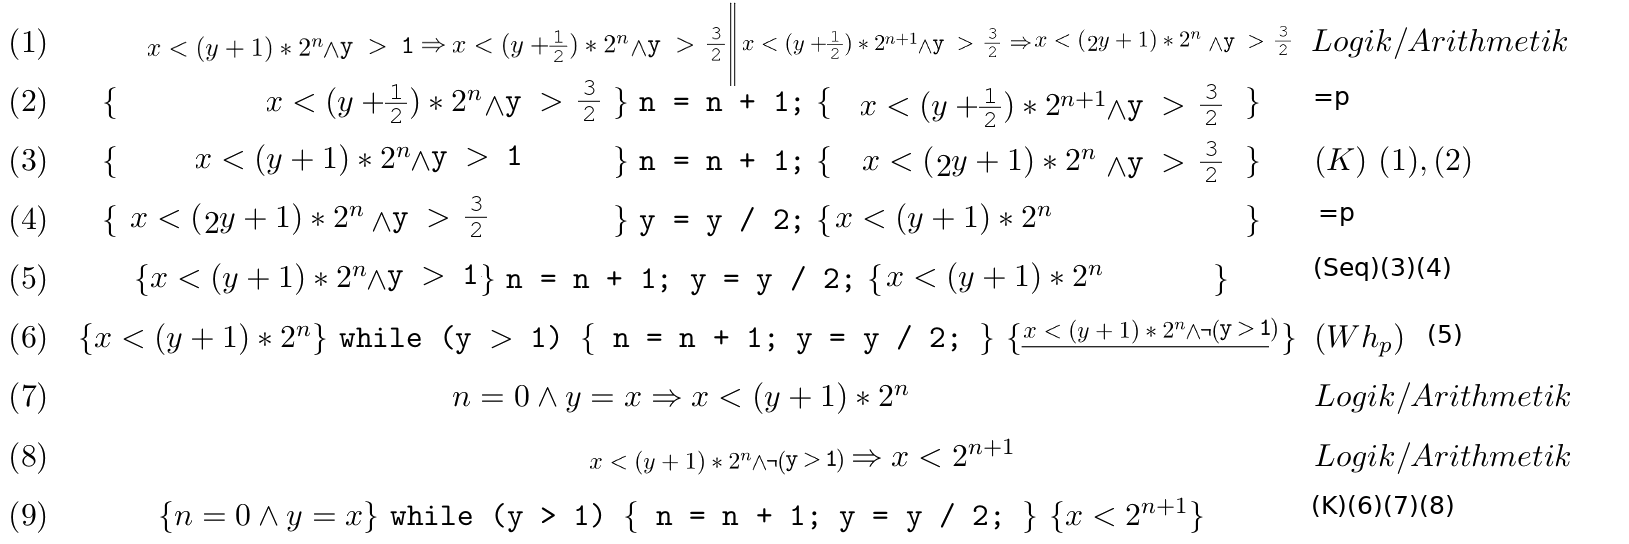
\includegraphics[width=1\textwidth]{a1.png}
\end{center}


\task{2}{6}
\begin{enumerate}[1.]
	\item Erfüllbar, mit Ablauf $(\{p,q\})^\omega$
	\item Erfüllbar, mit Ablauf $\{p\},\emptyset^\omega$
	\item Nicht erfüllbar, da $p \to \lnot p$ in keinem zustand erfüllt sein kann.
	\item Erfüllbar, mit Ablauf $(\{p\})^\omega$
\end{enumerate}


\task{3}{6}
\begin{enumerate}[1.]
	\item $\X\G p \models \G p$ ist nicht herleitbar, da für $(\emptyset, \{p\}^\omega)$ zwar $\X\G p$ erfüllt, aber nicht $\G p$. 
	\item \begin{align}
		\G p & \models \G p   & \in \text{M} \\
		\G p & \models \G\X p & \text{Folgt nach T3 aus} & \, (1)\\
		\G p & \models \X\G p & \text{Satz 5.2}          & \, (2)
	\end{align}
	\qed
	\item $\F(A\U B) \Rightarrow$ es existiert ein $i\geq 0$ mit $\pi^i \models A\U B \Rightarrow$ es existiert ein 
	$j\geq i$ mit $\pi^j\models B \Rightarrow \F B$. Die Rückrichtung gilt auch, da $A\U B$ auf für 
	$\pi = ({B},\emptyset^\omega)$ erfüllt ist (da in T4 auch $j=0$ gelten kann, und dann $0\leq i < j$ keine Elemente 
	enthält). Damit folgt aus $\F B$ auch $\F(A\U B)$.
	\qed
\end{enumerate}

\pagebreak 

\task{4}{4}
\begin{enumerate}[1.]
	\item \textbf{Abu ist der Täter}, Abu und Hasib haben gelogen. Jede andere Kombination macht keinen Sinn.
		  Wenn Abu nich gelogen hat, haben wir $\{H,\lnot H\}$. Wenn Hasib nicht gelogen hat, haben wir $\{H,A\}$, was 
		  auch nicht sein kann, da es nur einen Täter gibt.
	\item \textbf{Ibn ist der Täter}. Wenn Abu der täter wäre, hätten alle anderen gelogen, was laut vorraussetzung 
	nicht stimmmt. Wenn Hasib der Täter wäre, würde das Heißen, dass Ibn die Wahrheit sagt, dieser sagt aber, dass Hasib 
	nicht der täter ist. Wenn Ibn der Täter ist, dann lügt Abu, und Hasib sagt die Wahrheit.
	\item \textbf{Hasib ist der Täter}. Wenn Abu der Täter wäre, hätte Hasib gelogen, und Ibn, dessen Aussage den 
	NSU-Briefkasten genommen hat, wäre auch der Täter gewesen. Dies ist ein Wiederspruch. Wenn Ibn der Täter wäre, hätte 
	Abu gelogen, und Hasib wäre auch Täter. Nur wenn Hasib der Täter ist, und die Wahrheit sagt, dass Ibn nicht der Täter 
	war, und Abu lügt, geht alles auf. \emph{Weil das ja klar ist.} \qed
	\item \textbf{Hasib ist der Täter}. Da Abu und Ibn beide die Wahrheit sagen, müssen beide die gleich Person 
	beschuldigen. Da Aber niemand sich selbst beschulfigt, können sie nur Hasib beschuldigen. Deshalb muss Hasib der 
	Täter sein.
\end{enumerate}



\pointsttl{25}

\vfill\centering\includesvg[scale=.5]{../../smile.svg}
\end{document}
